\documentclass[a4paper, 12pt]{article}

\usepackage{sbc-template}
\usepackage[english]{babel}
\usepackage[utf8]{inputenc}
\usepackage[T1]{fontenc}
\usepackage{fontspec}
\usepackage{array}
\usepackage{fixltx2e}
\usepackage{amsmath}
\usepackage{amssymb}
\usepackage{graphicx}
\usepackage{float}
\usepackage{a4wide}
\usepackage{array}
\usepackage{multicol}
\usepackage[table]{xcolor}
\usepackage{makeidx}
\usepackage{hyperref}
\usepackage{booktabs}
\usepackage{setspace}
\usepackage[colorinlistoftodos,prependcaption,textsize=footnotesize]{todonotes}
\usepackage{minted}
\usepackage[bottom]{footmisc}
\usepackage[nottoc]{tocbibind}
\usepackage{listings}
\usepackage[a4paper]{geometry}
\usepackage[square, sort, comma, numbers]{natbib}

\onehalfspacing
\graphicspath{{./img/}}

\setcounter{secnumdepth}{2}
\setcounter{tocdepth}{2}

\setsansfont{DejaVu Sans}
\setmonofont{DejaVu Sans Mono}

\begin{document}

\hypersetup{backref,pdfpagemode=FullScreen,colorlinks=true}

\thispagestyle{empty}
\begin{center}
    \textbf{\Large{Program Autotuning with \\ Cloud Computing and OpenTuner}}\\

    \vspace*{0.5cm}

    \begin{minipage}{.3\linewidth}
        \begin{flushleft}
            Pedro Bruel\\
            phrb@ime.usp.br
        \end{flushleft}
    \end{minipage}
    \begin{minipage}{.3\linewidth}
        \begin{center}
            Alfredo Goldman\\
            gold@ime.usp.br
        \end{center}
    \end{minipage}
    \begin{minipage}{.3\linewidth}
        \begin{flushright}
            Daniel Batista\\
            batista@ime.usp.br
        \end{flushright}
    \end{minipage}

    \vskip 0.5cm

    \normalsize{Instituto de Matemática e Estatística (IME)\\
                Universidade de São Paulo (USP)\\
                R. do Matão, 1010 – Vila Universitária, São Paulo – SP, 05508-090\\}

\end{center}

\begin{abstract}
    The OpenTuner framework provides domain-agnostic tools for the
    implementation of autotuners. The optimization results are
    obtained sequentially by the measurement driver, that runs
    in a local machine.
    This paper presents an extension to the OpenTuner measurement driver,
    enabling it to leverage cloud computing resources
    from the Google Compute Engine (GCE). We compare the performance of
    our implementation using a diverse benchmark.
    \todo[inline,author=Pedro]{A very short summary of the results will be
    provided in the abstract.}
\end{abstract}

\section{Introduction} \label{sec:intro}

\todo[inline,author=Disclaimer]{This is a draft of the paper. The results and
implementations are not final or completed. Future versions will improve
the presentation and present results and conclusions. The maximum page count
for SBRC is 14 pages, and this document is 9 pages long.}

The program autotuning problem fits in the framework of the Algorithm Selection
Problem, introduced by Rice in 1976~\cite{rice1976algorithm}. The objective of
an autotuner is to select the best algorithm, or algorithm configuration, for
each instance of a problem.  Algorithms or configurations are selected
according to performance metrics such as the time to solve the problem
instance, the accuracy of the solution and the energy consumed.  The set of all
possible algorithms and configurations that solve a problem define a
\emph{search space}. Guided by the performance metrics, various optimization
techniques search this space for the algorithm or configuration that best
solves the problem.

\todo[inline,author=Pedro]{I removed the Algorithm Selection Problem figure.
It is marginally relevant for the paper's subject, but not needed to understand
the contributions and results. Should I re-include it?}

Autotuners can specialize in domains such as matrix
multiplication~\cite{bilmes1997phipac}, dense~\cite{whaley1998atlas} or
sparse~\cite{vuduc2005oski} matrix linear algebra, and parallel
programming~\cite{jordan2012multi}. Other autotuning frameworks provide more
general tools for the representation and search of program configurations,
enabling the implementation of autotuners for different problem
domains~\cite{ansel2014opentuner,hutter2009paramils}.

The main contribution of this paper is the implementation of an
extension to the OpenTuner framework~\cite{ansel2014opentuner} that
enables it to leverage cloud computing resources.
The interactions between the local and virtual machines (VM) follows
the client-server model. The local machine (LM) runs a measurement client that
requests results from various measurement servers running in virtual machines
hosted at the Google Compute Engine (GCE).
We compare the performance of our extension with the
unmodified framework in a diverse benchmark of applications, identifying
the problem domains that benefit from this cloud-based approach.

\todo[inline,author=Pedro]{Added hooks for the initials GCE, LM and VM.}
\todo[inline,author=Pedro]{I used \lq{}leverage\rq{} to implicitly say
\lq{}potentially speedup the autotuning process\rq{}, but this expression
will be improved in future revisions.}

The rest of the paper is organized as follows.
Section~\ref{sec:related} discusses related work.
Section~\ref{sec:ot} discusses the architecture of the OpenTuner framework.
Section~\ref{sec:ext} presents the architecture of the measurement driver
extension, the GCE interface and the application protocol
that mediates the interactions between \emph{MeasurementClient} and
\emph{MeasurementServer}s.
Section~\ref{sec:norm} discusses the result normalization strategies.
Section~\ref{sec:exp} describes the experiments performed and the
applications used in the benchmark.
Section~\ref{sec:results} discusses the results.
Section~\ref{sec:conclusion} concludes.

\section{Related Work} \label{sec:related}

Rice's conceptual framework~\cite{rice1976algorithm} formed the foundation
of autotuners in various problem domains.  In 1997, the PHiPAC
system~\cite{bilmes1997phipac} used code generators and search scripts to
automatically generate high performance code
for matrix multiplication. Since then, systems tackled different domains with a
diversity of strategies. Whaley \emph{et al.}~\cite{whaley1998atlas} introduced
the ATLAS project, that optimizes dense matrix multiply routines. The
OSKI~\cite{vuduc2005oski} library provides automatically tuned kernels for
sparse matrices. The FFTW~\cite{frigo1998fftw} library provides tuned C
subroutines for computing the Discrete Fourier Transform.  In an effort to
provide a common representation of multiple parallel programming models, the
INSIEME compiler project~\cite{jordan2012multi} implements abstractions for
OpenMP, MPI and OpenCL, and generates optimized parallel code for heterogeneous
multi-core architectures.

Some autotuning systems provide generic tools that enable the implementation of
autotuners in various domains. PetaBricks~\cite{ansel2009petabricks} is a
language, compiler and autotuner that introduces abstractions, such as the
\texttt{\footnotesize either...or} construct, that enable programmers to define
multiple algorithms for the same problem.  The ParamILS
framework~\cite{hutter2009paramils} applies stochastic local search methods
for algorithm configuration and parameter tuning.  The OpenTuner
framework~\cite{ansel2014opentuner} provides ensembles of techniques that
search spaces of program configurations. Bosboom \emph{et al.} and Eliahu use
OpenTuner to implement a domain specific language for data-flow
programming~\cite{bosboom2014streamjit} and a framework for recursive parallel
algorithm optimization~\cite{eliahu2015frpa}.

In a progression of papers~\cite{gupta2012exploring,gupta2014evaluating,gupta2013hpccloud},
Gupta \emph{et al.} provide experimental evaluations of the application of
cloud computing to high performance computing, describing which kind of
applications has the greatest potential to benefit from cloud computing.
Their work highlights small and medium scale projects as the main beneficiaries
of cloud computing resources.

\section{OpenTuner} \label{sec:ot}

OpenTuner search spaces are defined by \emph{Configurations}, that are composed
of \emph{Parameter} of various types. Each type has restricted bounds and
manipulation functions that enable the exploration of the search space.
OpenTuner implements ensembles of optimization techniques that
perform well in different problem domains. The framework uses
\emph{meta-techniques} to coordinate the distribution of resources
between techniques.
Results found during search are shared through a
database. An OpenTuner application can implement its own search
techniques and meta-techniques, making the ensemble more robust.
The source code is available\footnote{Hosted at GitHub:
\texttt{\scriptsize github.com/jansel/opentuner}} under the MIT License.

\begin{figure}[htpb]
    \centering
    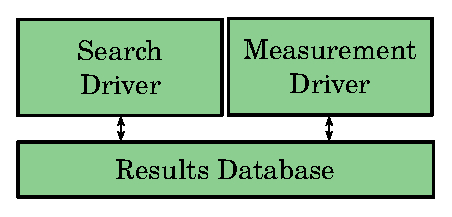
\includegraphics[scale=.62]{opentuner-implementation}
    \caption{Simplified OpenTuner Architecture.}
    \label{fig:ot-imp}
\end{figure}

Figure~\ref{fig:ot-imp} shows a high-level view of OpenTuner's architecture.
Measurement and searching are done in separate modules, whose main classes are
called \emph{drivers}. The search driver requests measurements by registering
configurations to the database. The measurement driver reads those
configurations and writes back the desired results.  Currently, the
measurements are performed sequentially.

OpenTuner implements optimization techniques such as the
Nelder-Mead~\cite{nelder1965simplex} simplex method and Simulated
Annealing~\cite{kirkpatrick1983optimization}. A resource sharing mechanism,
called \emph{meta-technique}, aims to take advantage of the strengths of each
technique by balancing the exploitation of a technique that has produced good
results in the past and the exploration of unused and possibly better ones.

\section{Measurement Server and Client}
\label{sec:ext}

Following the client-server model, the extension distributes
measurements of program configurations between a group of virtual
machines running \emph{MeasurementServer}s in the GCE. The servers
wait for measurement requests from a client. They maintain copies
of the program to be autotuned and the user-defined function that
measures configurations.

The machine running the OpenTuner autotuner runs a \emph{MeasurementClient},
an extension of the native \emph{MeasurementDriver} that, instead of
compiling and running requests locally, uses the GCE interface to
route requests to virtual machines and them saves the results to the local
database.

\begin{figure}[htpb]
    \centering
    \begin{minipage}{.45\textwidth}
        \centering
        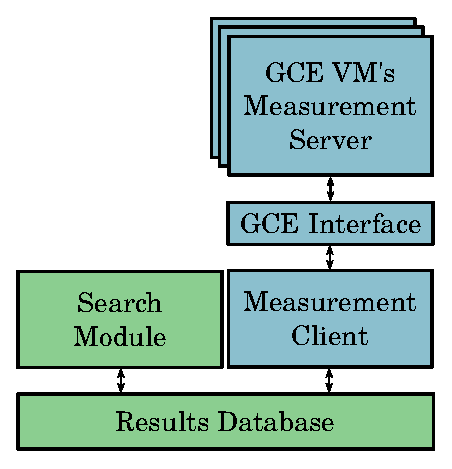
\includegraphics[scale=.58]{high-level-implementation}
        \caption{A high-level view of the architecture.}
        \label{fig:high-level}
    \end{minipage}%
    \hfill
    \begin{minipage}{.45\textwidth}
        \centering
        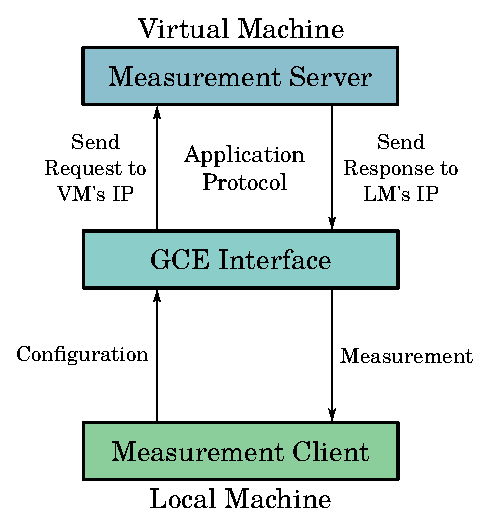
\includegraphics[scale=.58]{low-level-implementation}
        \caption{A lower-level view of the architecture.}
        \label{fig:low-level}
    \end{minipage}%
    \label{fig:archs}
\end{figure}

OpenTuner controls the execution flow of an application with the
\texttt{\footnotesize main} function of the \texttt{\footnotesize
TuningRunMain} class. This function sets up the database and the search and
measurement modules. It then calls the \texttt{\footnotesize main} function of
the search driver, which runs the main loop of the application.  The search
driver generates configurations to be tested and saves them to the database. It
then calls the \texttt{\footnotesize process\_all} function of the measurement
driver and blocks until the function returns.

\begin{listing}[htpb]
    \begin{minted}[fontsize=\scriptsize]{python}
class MeasurementClient(MeasurementDriver):
    """
    Reads DesiredResults and requests VMs
    in the cloud to compute Results.
    """
    def __init__(self,
           measurement_interface,
           input_manager,
           **kwargs):
        super(MeasurementDriver, self).__init__(**kwargs)
        """
        Now, the client will instantiate and 
        configure the VM Measurement Servers.
        """

    def process_all(self):
        """
        Process all results in the
        database, by sending requests to
        VMs in the cloud and waiting
        responses.
        """
    \end{minted}
    \caption{A simple echo server in Python.}
    \label{fig:measurement-client}
\end{listing}

\todo[inline,author=Pedro]{Listing 1 will be replaced by the complete
implementation if it is short enough. Otherwise it will be removed.}

The \texttt{\footnotesize process\_all} function is able to compile programs in
parallel, but the measurements are done sequentially.
Listing~\ref{fig:measurement-client} shows the functions of the measurement
driver that were modified to enable the \texttt{\footnotesize
MeasurementClient} to process results with Google Compute Engine resources.

Figure~\ref{fig:high-level} presents the architecture of an OpenTuner
application running the measurement client and communicating with the
measurement servers.  Green boxes in the figure represent OpenTuner modules
that will not be modified, and blue boxes represent new or modified modules.

Figure~\ref{fig:low-level} shows, on a lower level of abstraction, the
interactions between the measurement client and servers.
The client sends the program configurations to the servers, who run the
correspondent program and respond with the measurement.

During initialization the measurement client uses the GCE interface to start
and configure virtual machines. The interface stores each measurement
server's IP.  When the search driver makes requests for results, the
\texttt{\footnotesize process\_all} function will route them to the servers via
the GCE interface.  The interface will call the appropriate GCE Python API
functions, and wait for the responses.

\subsection{GCE Interface}
\label{sec:gce}

\todo[inline,author=Pedro]{This section will describe how the GCE interface
mediates the result requests and configuration measurements.}

The interactions between the local \emph{MeasurementClient} and the virtual
machines' \emph{MeasurementServer}s are mediated by a wrapper of the
GCE Python API, described in Section~\ref{sec:gce}.

The utility functions and the measurement server's and client's code are
available\footnote{All code is hosted at GitHub: \\ \texttt{\scriptsize
github.com/phrb/measurement-server} \\ \texttt{\scriptsize
github.com/phrb/autotuning-gce}} under the GNU General Public License.

\subsection{Application Protocol}
\label{sec:app}

\todo[inline,author=Pedro]{The application protocol will be described here.}

\section{Result Normalization}
\label{sec:norm}

\todo[inline,author=Pedro]{This section will discuss the different strategies
in more depth, and relate them to the experiments performed.}

Using a cloud environment, an autotuner will typically optimize programs for
a machine with a different architecture from the virtual machines. A
normalization technique must be devised that enables the results found in the
virtual machines to be valid for the local machine.  We present four
approaches to this problem. The best approach for each problem domain
must be experimentally determined, and could be a combination of the approaches
described here.

\paragraph{Autotune Performance Models}
Another autotuner could be implemented to optimize parameters of a simple
performance model, that would associate a configuration's measurement and the
virtual machine that produced it with a conversion function that transposes
performance results to the target architecture.

\paragraph{Ensembles of Virtual Machines}
The cloud application could be composed of virtual machines with different
architectures. The final performance measurement for a configuration would be
built from some combination of the results obtained in these different virtual
machines.

\paragraph{Architecture Simulators}
The target machine could be modeled by an architecture simulator such as
\emph{zsim}~\cite{sanchez2013zsim}, a simulator for multi-core architectures
available\footnote{Hosted at GitHub: \texttt{\scriptsize
https://github.com/s5z/zsim}} under the GNU General Public License.  Using a
simulator would solve the normalization problem but introduce other problems,
such as the simulator's accuracy and performance.

\paragraph{Autotune in the Cloud}
Finally, the normalization problem could be sidestepped, at least in initial
stages of research, by running the servers and clients in the cloud using
the same kind of virtual machine.

\section{Experiments} \label{sec:exp}

\todo[inline,author=Pedro]{The experimental settings will be described in this
section.}

\section{Results} \label{sec:results}

\todo[inline,author=Pedro]{This section will present and discuss the results, 
connecting the findings with normalization techniques and problem domains.}

\section{Conclusion} \label{sec:conclusion}

This paper presented an extension of the OpenTuner autotuning framework
enabling it to leverage the cloud computing resources from GCE.  We propose
four approaches to solve the result normalization problem which would enable
transposing the results obtained in virtual machines to a local machine.

\bibliographystyle{IEEEtran}
\bibliography{IEEEabrv,ref}

\end{document}
